%
% CRM.tex
% Customer Relations Management
%
% Aleph Objects Operations Manual
%
% Copyright (C) 2014, 2015 Aleph Objects, Inc.
%
% This document is licensed under the Creative Commons Attribution 4.0
% International Public License (CC BY-SA 4.0) by Aleph Objects, Inc.
%


\section{Helpdesk}
\begin{itemize}
\item Customer Support Representative (CSR): The front-line person who deals with the customer calls or emails.

\end{itemize}

\subsection{Requests Through Support Email}

Emails to support@alephobjects.com are directly registered in OpenERP as Helpdesk request. The process to handle these is as follows:

\begin{enumerate}
\item Customer support person logs into OpenERP and opens the Helpdesk requests list by going to Sales/After-Sale Services/Helpdesk and Support.
\item By default, only the active items (new, pending, in progress) are shown in the list.

  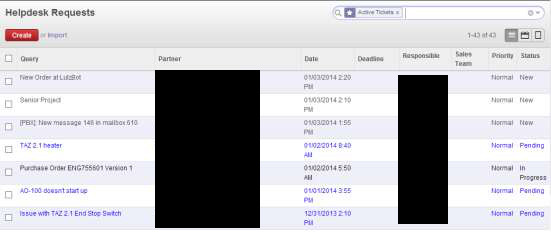
\includegraphics[keepaspectratio=true,angle=0,height=1.00\textheight,width=1.00\textwidth]{openerp/crm.jpg}
  
\item Additional filters can be applied using the search / filter feature in OpenERP.
\item Open the Helpdesk request (or ticket hereafter).
\item Review the request and take appropriate action
  \begin{enumerate}
  \item If the request is for information or a simple issue that can be resolved by the customer support person, do so.
    \begin{enumerate}
    \item Assign self as “Responsible” person on the ticket.
    \item Record the resolution in the “send a message”
    \item Email with the resolution will be sent to the requester
    \item Set Reference field to “Product” and select a product (typically a printer – e.g. TAZ Printer 2.0)
    \item Click on “Open” to set the state to “In Progress” and save the ticket.
    \end{enumerate}
  \item If the request needs to be worked upon before resolution, assign the request to appropriate person for resolution.
    \begin{enumerate}
    \item Assign the person
    \item Set category of the problem
    \item Set priority for the problem resolution
    \item Set Reference field to “Product” and select a product (typically a printer – e.g. TAZ Printer 2.0)
    \item Click on “Open” to set the state to “In Progress” and save the ticket.
    \item If required, send an email to the reporter by using “Send a message” from the chatter area (the area below the Helpdesk request form).
    \item Use “Log a note” if you wish to record your observations / queries to the responsible person working on the ticket. This information will be retained internally and will not be emailed to the reporter.
Note: If the request is based on an order (sale order, delivery order), then use the Reference2 field to pick the sale order / delivery order and select the sale order for the customer reporting the problem.
    \end{enumerate}
  \end{enumerate}
\item Reviewing In-Progress/Pending items: Periodically review these tickets and provide updates to the customer by using “Send a message.”
\item Closing tickets: Once the resolution is accepted by the customer (you may not hear the success of the resolution from the customer always – so closing resolved cases after a gestation period is OK). If the customer responds to a resolution on a closed ticket, the ticket will be reopened for your review automatically allowing the ticket to be reopened or closed/cancelled.
\item Cancelling tickets: If the ticket is a spam or made for testing purposes, it can be cancelled by clicking on the Cancel Case button.
\end{enumerate}


\subsection{Requests through Phone / Direct Email}

The only difference in this is that the Helpdesk request (ticket) does not exist in the system and so it must be created.
\begin{enumerate}
\item On receiving a phone call from a customer,  customer support person logs into OpenERP and opens the Helpdesk requests list by going to Sales/After-Sale Services/Helpdesk and Support. 
\item Click on Create button to create a new request.
\item Select the partner from the list of available partners. If the call is from a person not registered as a customer with Aleph Objects, record the information in the notes section – name, phone number, address and other pertinent details of the customer.
\item Record the email address of the caller. 
\item Write a brief summary header in the “Query” field.
\item Based on your assessment of the call, set the priority of the call and the category.
\item Continue processing the ticket following the procedure outlined for the automated email (to support@alephobjects.com) ticket.
Note: Process Helpdesk requests in personal emails in the same manner as a call.
\end{enumerate}

\section{Using the Phones}
See: \texttt{shared-j/Documents/phone\_directory.txt} for the most current
company phone directory.

\subsection{Transfer call}
\begin{enumerate}
\item Ask the caller if you can transfer them.
\item Put the call on hold: *2
\item Dial internal extension number you want to transfer to.
\item Explain transfer when internal callee answers.
\item Hang up, and the call will automatically transfer.
\end{enumerate}

\section{Forum}
Answer questions and contribute information at our LulzBot forum:
\texttt{http://forum.lulzbot.com/}

\section{RMA}
Return Merchanise Authorization. Through OpenERP.

\section{Chat}
Chat server at
\texttt{jabber.alephobjects.com}
